\documentclass[12pt, twoside]{article}
\usepackage[francais]{babel}
\usepackage[T1]{fontenc}
\usepackage[latin1]{inputenc}
\usepackage[left=1Cm, right=1cm, top=1Cm, bottom=1Cm]{geometry}
\usepackage{float}
\usepackage{graphicx}
\usepackage{array}
\usepackage{multirow}
\usepackage{amsmath,amssymb,mathrsfs}
\usepackage{soul}
\pagestyle{empty}

\begin{document}

\begin{flushright}
$2^{de}5$
\end{flushright}
\begin{center}
\textbf{\large{Devoir Maison 4}}
\end{center}

\textit{Devoir � rendre sur feuille double grand format petits carreaux pour le
\ul{samedi 22 novembre 2008}.}

\textit{La qualit� de la r�daction et de la pr�sentation sont prises en compte
dans la notation.}



\bigskip
\textbf{Exercice 1:} (\textit{6,5 points})

\begin{tabular}{cc}
\begin{minipage}{9cm}
\begin{center}
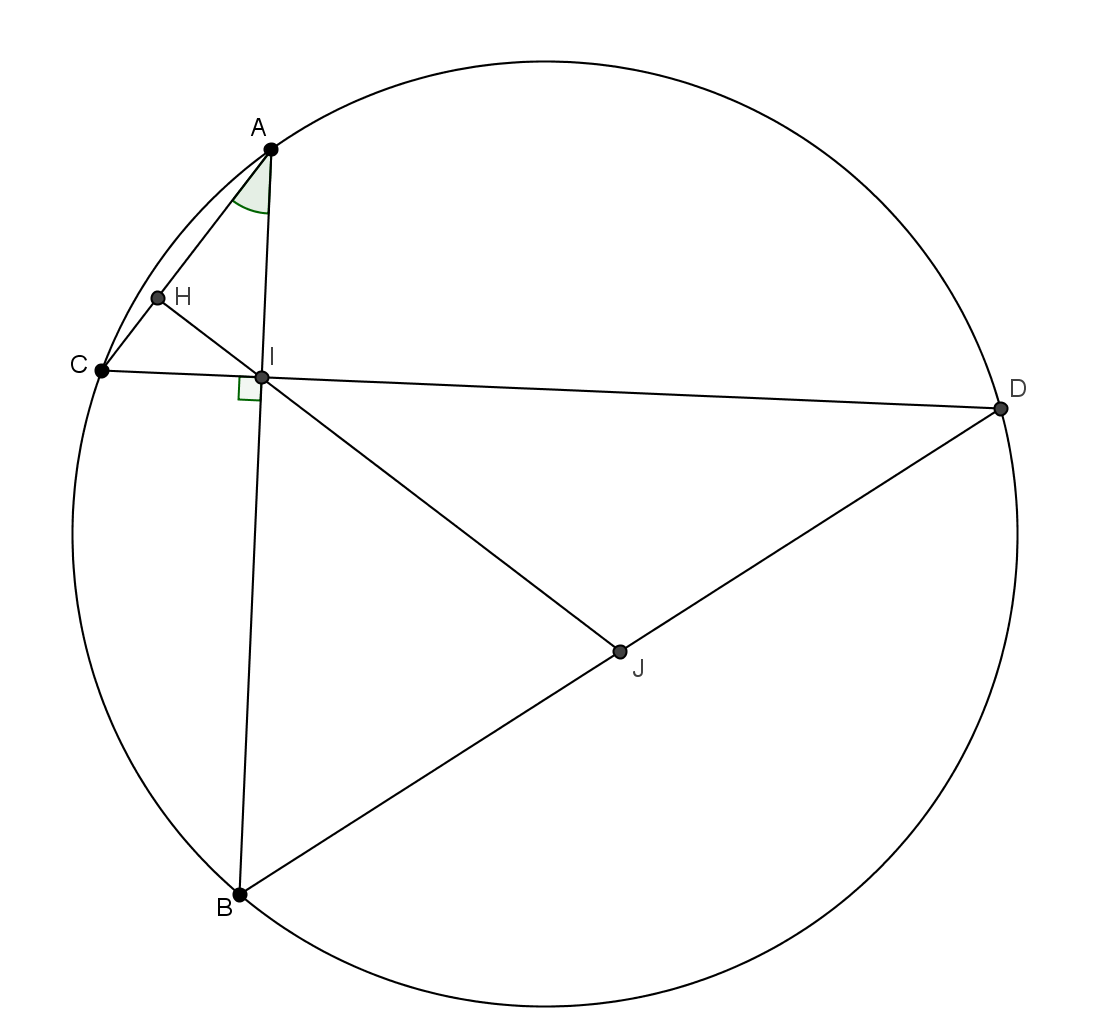
\includegraphics[width=8cm]{image/geogebra.png}
\end{center}
\end{minipage}
&
\begin{minipage}{8cm}
Sur la figure ci-contre, $A,B,C,D$ sont quatre points d'un cercle tels que les
droites $(AB)$ et $(CD)$ soient perpendiculaires. On note $I$ le point
d'intersection. Le point $J$ est le milieu du segment $[BD]$ et la droite $(IJ)$
coupe le segment $[AC]$ en $H$. L'angle $\widehat{IAC}$ mesure $35$�.

\end{minipage}
\end{tabular}
  




\medskip

\fbox{ \begin{minipage}{18cm}
         
Lors du pr�c�dent devoir, � l'aide de g�og�bra, nous avons trouv�
que \textbf{l'angle $\widehat{IHA}$ est un angle droit}. Le but de l'exercice
est de d�montrer cette conjecture.
 \end{minipage}
}

\begin{enumerate}
  \item Montrer que $\widehat{IDB}=35�$.
  \item Montrer que l'angle $\widehat{IHA}$ est un angle droit.
\end{enumerate}

\bigskip
\bigskip


\textbf{Exercice 2:} (\textit{6 points})


R�diger soigneusement l'exercice commenc� le samedi 15 novembre (un partage
�quitable).


\begin{center}
\fbox{Pour cet exercice, vous serez �valu�s en grande partie sur la
r�daction de votre travail.}
\end{center}

\bigskip
\bigskip

\textbf{Exercice 3:} (\textit{5,5 points})


R�soudre les �quations et in�quations suivantes:
\begin{enumerate}
  \item $|x-4|=3$
  \item $|x+1|<4$
  \item $|x+2|=|2-x|$
  \item $|x-3| \geqslant |x+2|$
\end{enumerate}


\bigskip
\bigskip


\textbf{Exercice 4:} (\textit{3 points dont UN BONUS})

\begin{enumerate}
  \item Ecrire $\sqrt{(1-\sqrt{3})^{2}}$ sans racines carr�es.
  \item Soit $y$ un nombre r�el. Ecrire $\sqrt{(4y^{2}-12y+9)^{2}}$ sans racines
  carr�es (\textit{Indication:} diff�rencier les cas selon les valeurs de $y$).
\end{enumerate}

\end{document}
